\subsection{Optimierung}
%\label{subsection:Optimierung}
Im Projekt wurden drei Optimierungen vorgenommen, um die Laufzeit des Programms zu verkürzen.\\

\subsubsection{Optimierungsschritt}
Um die Laufzeit des Programms zu verkürzen, werden entgegen einer ersten Implementierung nicht einzelne Zeichen, welche ein Wort bilden verschickt, sondern ein Array mit allen Zeichen bzw. Wörtern zusammengesetzt. Um zu verdeutlichen, aus welchen Zeichen ein Wort besteht, wird zwischen den Wörter ein Semikolon eingefügt. Dadurch kann ein Slave-Knoten aus dem Array die Wörtern rekonstruieren. Dies führt zu einer Optimierung der Laufzeit, da die laufzeitintensiven Befehle \textit{MPI\_Send()} und \textit{MPI\_Recv()} nicht mehr nach jedem Zeichen ausgeführt werden sondern nur noch einmal pro Prozess. \\
Wenn die Zeichen aus der einzulesenden Datei einzeln verschickt werden, finden bei einer Beispieldatei mit ca. 400.000 Wörtern etwa 2.500.000 Aufrufe der Funktionen \textit{MPI\_Send()} und \textit{MPI\_Recv()}. Zusätzlich werden auch beim Rücksenden der einzelnen Zeichen an den Master ca. 2.500.000 Aufrufe der beiden Funktionen benötigt.\\
Nach der Optimierung waren Verbesserungen der Laufzeit zu beobachten. Zwei Prozesse benötigen mit der Optimierung etwa 2,5 Sekunden zum Sortieren. Vor der Optimierung lag die Laufzeit bei bei etwa 6 Sekunden. 

\subsubsection{Optimierungsschritt}
Im Programmentwurf versendet der Master-Knoten die Wörter an die sieben Prozesse zum Sortieren, ohne selber einen Bereich zu sortieren. Dies führt dazu, dass ein Prozess nur die Daten verschickt und empfängt. In der Zwischenzeit, wo die sieben Prozesse sortieren, wartet ein Prozess bis Daten zurückgeschickt werden. Diese Zwischenzeit kann der Master nutzen, um selber einen Teilbereich zu sortieren. So werden acht statt sieben Prozesse zum Sortieren genutzt.  

\subsubsection{Optimierungsschritt}
\label{Optimierung3}
Eine weiterer Optimierungsschritt ist, dass alle eingelesenen Wörter aus der Datei in einem Array verschickt werden. Somit muss der Array zunächst nicht in die einzelnen zu sortierenden Bereiche aufgeteilt werden. In Abbildung \ref{fig:Ooptimierung} wird verdeutlicht, dass alle Prozesse den selben Ausgangsarray vom Master erhalten \\
Jeder Prozess erhält einen Buchstabenbereich von 3 Buchstaben, z.B. wird dem erste Prozess der Buchstabenbereich von a bis c zugeordnet. Somit sortiert er nur die Wörter alphabetisch, die mit a, b oder c beginnen.
Die wesentliche Optimierung liegt am Zusammenführen der einzeln sortierten Arrays. 
Die sortierten Teilarrays werden an den Master zurückgesendet. Wie in Abbildung \ref{fig:Ooptimierung} fügt der Master die sortierten Arrays hintereinander zu einem vollständig sortieren Array zusammen. Hierbei wird die Durchführung des \textit{merge\_back()} beim Master eingespeichert, wo er miteinander vergleicht und sortiert. \\


\begin{figure}[htbp]
	\centering

	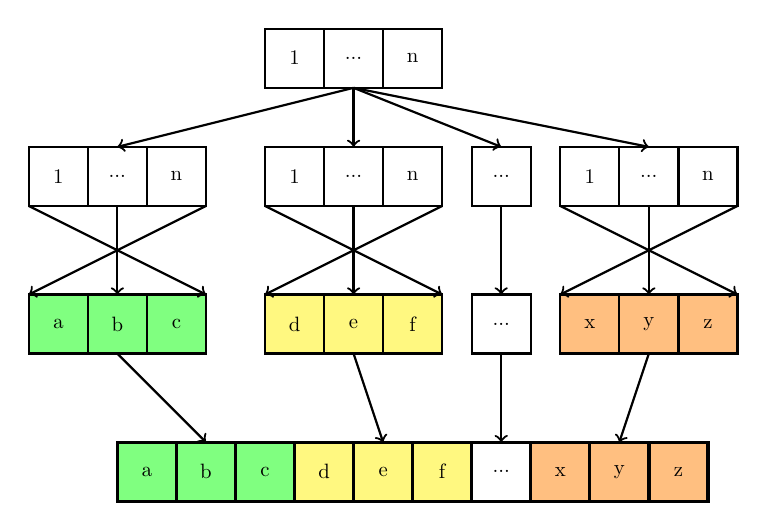
\begin{tikzpicture}[scale=0.75, transform shape]
	\draw [thick] (1,6.5) rectangle(2,7.5) node[pos=.5]{1};
	\draw [thick] (2,6.5) rectangle(3,7.5) node[pos=.5]{...};
	\draw [thick] (3,6.5) rectangle(4,7.5)node[pos=.5]{n};
	
	\draw [thick] (-3,4.5) rectangle(-2,5.5)node[pos=.5] {1};
	\draw [thick] (-2,4.5) rectangle(-1,5.5)node[pos=.5] {...};
	\draw [thick] (-1,4.5) rectangle(0,5.5)node[pos=.5] {n};
	
	\draw [thick] (1,4.5) rectangle(2,5.5)node[pos=.5] {1};
	\draw [thick] (2,4.5) rectangle(3,5.5)node[pos=.5] {...};
	\draw [thick] (3,4.5) rectangle(4,5.5)node[pos=.5] {n};
	
	\draw [thick] (4.5,4.5) rectangle(5.5,5.5)node[pos=.5] {...};
	
	\draw [thick,] (6,4.5) rectangle(7,5.5)node[pos=.5] {1};
	\draw [thick] (7,4.5) rectangle(8,5.5)node[pos=.5] {...};
	\draw [thick] (8,4.5) rectangle(9,5.5)node[pos=.5] {n};
	
	
	\draw [thick, fill=green!50] (-3,2) rectangle(-2,3)node[pos=.5] {a};
	\draw [thick, fill=green!50] (-2,2) rectangle(-1,3)node[pos=.5] {b};
	\draw [thick, fill=green!50] (-1,2) rectangle(0,3)node[pos=.5] {c};
	
	\draw [thick, fill=yellow!50] (1,2) rectangle(2,3)node[pos=.5] {d};
	\draw [thick, fill=yellow!50] (2,2) rectangle(3,3)node[pos=.5] {e};
	\draw [thick, fill=yellow!50] (3,2) rectangle(4,3)node[pos=.5] {f};
	
	
	\draw [thick] (4.5,2) rectangle(5.5,3)node[pos=.5] {...};
	
	\draw [thick, fill=orange!50] (6,2) rectangle(7,3)node[pos=.5] {x};
	\draw [thick, fill=orange!50] (7,2) rectangle(8,3)node[pos=.5] {y};
	\draw [thick, fill=orange!50] (8,2) rectangle(9,3)node[pos=.5] {z};

	
	\draw [very thick, fill=green!50] (-1.5,-0.5) rectangle(-0.5,0.5)node[pos=.5] {a};
	\draw [very thick, fill=green!50] (-0.5,-0.5) rectangle(0.5,0.5)node[pos=.5] {b};
	\draw [ very thick, fill=green!50] (0.5,-0.5) rectangle(1.5,0.5)node[pos=.5] {c};
	\draw [ very thick, fill=yellow!50] (1.5,-0.5) rectangle(2.5,0.5)node[pos=.5] {d};
	\draw [very thick, fill=yellow!50] (2.5,-0.5) rectangle(3.5,0.5)node[pos=.5] {e};
	\draw [very thick, fill=yellow!50] (3.5,-0.5) rectangle(4.5,0.5)node[pos=.5] {f};
	\draw [ very thick] (4.5,-0.5) rectangle(5.5,0.5)node[pos=.5] {...};
	\draw [ very thick, fill=orange!50] (5.5,-0.5) rectangle(6.5,0.5)node[pos=.5] {x};
	\draw [ very thick, fill=orange!50] (6.5,-0.5) rectangle(7.5,0.5)node[pos=.5] {y};
	\draw [ very thick, fill=orange!50] (7.5,-0.5) rectangle(8.5,0.5)node[pos=.5] {z};
	
	\draw [thick,draw=black,->] (2.5,6.5) -- (-1.5,5.5);
	\draw [thick,draw=black,->] (2.5,6.5) -- (2.5,5.5);
	\draw [thick,draw=black,->] (2.5,6.5) -- (5,5.5);
	\draw [thick,draw=black,->] (2.5,6.5) -- (7.5,5.5);
	
	\draw [thick,draw=black,->] (-3,4.5) -- (0,3);
	\draw [thick,draw=black,->] (-1.5,4.5) -- (-1.5,3);
	\draw [thick,draw=black,->] (0,4.5) -- (-3,3);
	
	\draw [thick,draw=black,->] (1,4.5) -- (4,3);
	\draw [thick,draw=black,->] (2.5,4.5) -- (2.5,3);
	\draw [thick,draw=black,->] (4,4.5) -- (1,3);
	
	\draw [thick,draw=black,->] (5,4.5) -- (5,3);
	
	\draw [thick,draw=black,->] (6,4.5) -- (9,3);
	\draw [thick,draw=black,->] (7.5,4.5) -- (7.5,3);
	\draw [thick,draw=black,->] (9,4.5) -- (6,3);
	
	\draw [thick,draw=black,->] (-1.5,2) -- (0,0.5);
	\draw [thick,draw=black,->] (2.5,2) -- (3,0.5);
	\draw [thick,draw=black,->] (5,2) -- (5,0.5);
	\draw [thick,draw=black,->] (7.5,2) -- (7,0.5);
	

	\end{tikzpicture}
	\caption[3.Optimierungsschritt]{Darstellung des dritten Optimierungsschritts. Hier werden die einzelnen Schritte des Ausgangsarray bis zum sortierten Array dargestellt.Der Master fügt die sortieren Teilarrays am Ende zusammen.}
	\label{fig:Ooptimierung}
\end{figure}

%Mögliche Optimierung (wenn nicht gewünscht weglassen)
\subsection{Optimierter Algorithmus}
Zusätzlich zu den Optimierungen am bestehenden Algorithmus wird eine alternative Aufteilung und Sortierung der Daten erarbeitet. Anstatt den initialen Vektor von einem Master Knoten aus auf eine beliebige Anzahl Worker aufzuteilen, kann eine Baumstruktur erstellt werden. Dabei sendet ein Ursprungsknoten die Hälfte des Datensatzes an einen weiteren Knoten. Diesen Prozess setzt jeder Knoten unabhängig fort, bis alle Rechenknoten verwendet werden. Anschließend führt jeder Knoten die Sortierung durch und sendet den sortierten Vektor wieder an den Knoten zurück, von welchem der Vektor empfangen wurde. Dieser Knoten führt durch die bestehende Funktion des Merge-Sorts die beiden sortierten Vektoren in einen sortierten Vektor zusammen und sendet diesen wiederum an den nächsthöheren Knoten. Dieser Prozess wird wiederholt, bis der Urpsrungsknoten die gesamten Daten hat. Das Ergebnis ist ein sortierter Vektor. Es werden hierbei nicht nur die Sortierungen Parallelisiert, sondern auch das Versenden sowie das Zusammenführen der Daten. Die gleichzeitige Ausführung von mehreren Prozessen sorgt dabei für eine bessere Ausnutzung der verfügbaren Rechenkapazitäten. Aufgrund von begrenzter Projektzeit wird dieser Algorithmus im Rahmen dieser Arbeit nicht implementiert oder getestet.
\begin{figure}[!t]
	\centering
	\includegraphics[width=3.5in]{Parallelisierungs_Algorithmus_2.png}
	\caption{Beispielhafter Durchlauf des Algorithmus mit 5 Nodes}
	\label{para_algo2}
\end{figure}